\RequirePackage[T1]{fontenc}
\documentclass[10pt,journal,letterpaper]{IEEEtran}
\usepackage{amsmath,amssymb,amsthm,booktabs,array,microtype}
\usepackage[hidelinks]{hyperref}
\usepackage{fancyhdr,tikz,graphicx}
\usetikzlibrary{arrows.meta}
\hypersetup{pdftitle={Exceeding Virtual Stable Storage on Commodity Hardware},pdfauthor={Simon Massey}}
\newcommand{\paperrevision}{RESEARCH CHECKPOINT --- 19 SEPTEMBER 2026}
\newcommand{\paperversion}{DRAFT}
\IfFileExists{version.tex}{\input{version.tex}}{}
\pagestyle{fancy}
\fancyhf{}
\fancyhead[R]{\footnotesize\thepage}
\fancyfoot[C]{\scriptsize\paperrevision\ --- \paperversion}
\renewcommand{\headrulewidth}{0pt}
\setlength{\emergencystretch}{1em}
\raggedbottom
\newtheorem{theorem}{Theorem}
\newtheorem{lemma}{Lemma}
\newtheorem{proposition}{Proposition}
\newcommand{\code}[1]{\texttt{#1}}
\title{Exceeding Virtual Stable Storage\\on Commodity Hardware}
\author{Simon Massey\thanks{Author draft. Correspondence: simon.massey@stenographer.cloud.}}
\begin{document}
\maketitle
\thispagestyle{fancy}

\begin{abstract}
Virtual stable storage repairs the diskless crash recovery of Viewstamped
Replication Revisited by replacing each write to stable storage with a write
to a quorum of processes: a push round-trip inserted into the fencing path of
the transformed protocol, paid once per fenced action and again at every
recovery. This paper presents the alternative reading of Unbounded
Viewstamped Replication Revisited (uVRR). Read as a repair of Viewstamped
Replication it looks like the heavier construction; read as a design point
for agreement over small metadata on commodity hardware it exceeds the
virtual-stable-storage construction it is measured against. uVRR makes a
crash final for the protocol identity: the fence and the voter share a
lifetime, so no quorum round is spent carrying a fence across a crash, and no
disk flush sits on the replication path. Local durable writes survive only at
lifecycle boundaries --- a clean stop, a boot --- where a
TigerBeetle-derived superblock discipline of spaced direct copies and a
four-state marker machine lets the boot decide clean from dirty with local
sector reads alone. The design retires a cost the literature has moved
between disk and network since 1988 without removing it.
\end{abstract}

\begin{IEEEkeywords}
Crash-stop, diskless recovery, stable storage, strong consistency, Viewstamped Replication.
\end{IEEEkeywords}

\section{Introduction}\label{sec:intro}
The fencing of a replicated view has been paid for three times over, in three
currencies, and the literature records each payment as progress.
The 1988 Viewstamped Replication of Oki and Liskov paid it in disk: a replica
records its view fence on local stable storage before its report is
released~\cite{vr}.
The 2012 Viewstamped Replication Revisited (VRR) of Liskov and Cowling declined to
pay, keeping the fence volatile; Michael \emph{et al.}\ showed in 2016 that
the corresponding recovery is unsafe, because a replica can forget a
view-change commitment it has already sent and vote again in a stale
view~\cite{diskless}.
Their repair, virtual stable storage, pays the fence in network: every write
to stable storage becomes a write to a quorum of processes, a push round-trip
on the fencing path of the transformed protocol~\cite{diskless}.
The TigerBeetle production design pays it in disk again, with rigour: four
spaced superblock copies, a hash-chained sequence, and a double journal
write, flushed on the request path of a financial ledger~\cite{tigerbeetle}.
Each design moves the cost. None removes it.

Unbounded Viewstamped Replication Revisited (uVRR) removes it, and the
removal is easy to miss because the construction is usually described as a
repair of VRR~\cite{uvrr}.
A crash is final for the protocol identity: the crashed identity never
resumes, the process rejoins under a fresh identity as a non-voting standby,
and voting authority arrives through committed membership changes.
The unsafe vote of the VRR counterexample is then unrepresentable rather than
filtered: there is no identity left to cast it.
Nothing about that argument requires a fence to survive a crash, because the
voter that could forget the fence does not survive the crash either.
The fence and the voter share a lifetime, and the fencing tax --- disk write,
push round-trip, or hot-path flush --- is retired with the voter.

This paper states the design point in storage terms and prices it against the
construction it exceeds.
Section~\ref{sec:cost} prices virtual stable storage honestly: its cost is
not disk traffic but a synchronous quorum round-trip inserted into the
fencing path, per fence, forever.
Sections~\ref{sec:reincarnation} and~\ref{sec:storage} describe uVRR's
identity finality and the local storage discipline that distinguishes a clean
stop from a crash on commodity hardware.
Section~\ref{sec:ledger} sets the ledger; Section~\ref{sec:soundness} states
the soundness conditions; Section~\ref{sec:scope} states where the claim does
not hold.

\begin{figure*}[t]
\centering
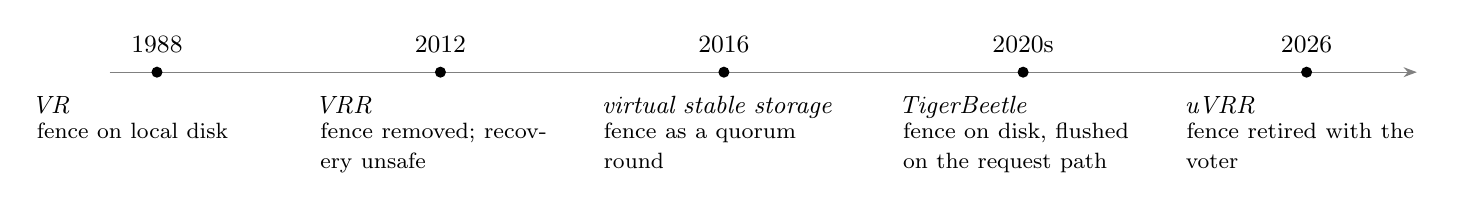
\begin{tikzpicture}[x=1cm,y=1cm,>=Stealth,font=\small]
\draw[->,gray] (0,0)--(16.6,0);
\foreach \x/\yr/\name/\paid in {
  0.6/1988/{VR}/{fence on local disk},
  4.2/2012/{VRR}/{fence removed; recovery unsafe},
  7.8/2016/{virtual stable storage}/{fence as a quorum round},
  11.6/2020s/{TigerBeetle}/{fence on disk, flushed on the request path},
  15.2/2026/{uVRR}/{fence retired with the voter}%
}{
  \fill (\x,0) circle (2pt);
  \node[anchor=south] at (\x,0.12) {\yr};
  \node[anchor=north,align=left,text width=3.05cm] at (\x,-0.18) {\textit{\name}\\[-2pt]\footnotesize \paid};
}
\end{tikzpicture}
\caption{The fencing cost moved, never removed. Time is not to scale.}
\label{fig:arc}
\end{figure*}

\section{The cost model of virtual stable storage}\label{sec:cost}
Virtual stable storage is a general transformation: any protocol correct in
the crash-stop or crash-recovery-with-stable-storage model is transformed
into one correct in the diskless crash-recovery model by replacing each write
to stable storage with an acquisition of a quorum~\cite{diskless}.
The write terminates when replies arrive from a strict majority; the
receiving processes add the written value to their volatile sets; a crash
vector per process detects when a replying process has crashed and recovered,
and stale replies are discarded and the request repeated.
Recovery is the same acquisition with an empty value, and a recovering
process is not operational --- may not resume its protocol --- until its
quorum round completes.

Three properties of this construction fix its price.

\emph{The fence costs a push round-trip, per fence, forever.}
Whatever a protocol would persist, the transformed protocol persists by
synchronous communication with a majority.
For Viewstamped Replication the persisted item is the view fence: the 1988
disk write that precedes the release of a view-change report~\cite{vr}.
Under the transformation that write becomes a quorum round on the fencing
path of every view change at every replica.
The normal path stays as cheap as VRR's; the fencing path, the path that must
complete before a new view may form, carries the tax.
Under churn the round lengthens: replies from processes that crash
mid-exchange are discarded and the acquisition is retried.

\emph{Recovery costs a push round-trip before the process may vote.}
A crashed process returns only by acquiring a quorum, and only operational
processes reply.
The recovering process contributes no vote during its recovery, exactly as a
uVRR standby contributes none during its catch-up; the two designs are at
parity here, and the parity is worth stating because it isolates the
difference, which is the fencing tax above.

\emph{Durability is the liveness of the quorum.}
The store is memory only.
If a majority is ever simultaneously down or recovering, no process can
acquire a quorum again: no write completes and no recovery terminates, ever
after~\cite{diskless}.
To keep the fencing round cheap the quorum must sit within a datacentre; to
keep the store alive that quorum must never fail together.
The construction buys freedom from disk failure by concentrating the failure
domain into quorum liveness, and the commodity intra-datacentre network is
what makes the round affordable at all~\cite{netdisk}.

None of this is a criticism: as a general transformation with proofs of
persistence and termination, virtual stable storage is the reference design
for diskless crash recovery, and its counterexample is what makes VRR's
recovery precise enough to exceed.
The claim here is narrower and stronger: for agreement over small metadata on
commodity hardware, none of the three payments above is necessary.

\section{Crash-stop reincarnation}\label{sec:reincarnation}
uVRR retains VRR's volatile normal path and its two-phase view change
unchanged~\cite{vrr,uvrr}.
What changes is the meaning of a crash.
A crashed identity never resumes execution.
The process that replaces it joins under a fresh identity with voting weight
zero: a standby that cannot form part of any quorum.
Its catch-up --- a quorum read and state transfer --- runs outside the voting
protocol while it cannot vote, and its promotion to voting weight is itself a
committed membership change, organised across the configuration boundary by
leader overlap~\cite{turner,uvrr}.
Messages sent before the crash remain messages of the old identity; the
mechanised development proves that a superseded identity casts no vote in any
later configuration~\cite{uvrr,artifact}.

The consequence for the fencing question is direct.
VRR's recovery had to restore two things at once: the replica's data and the
commitments of its identity --- the view fences it had already sent.
Virtual stable storage restores both by repairing the voter's memory.
uVRR restores the data and declines to restore the identity: the commitments
of the crashed identity die with it, and the replacement has no commitments
to honour because it has sent nothing.
The fence that 1988 wrote to disk and 2016 wrote to a quorum is, in uVRR,
never written at all.
There is nothing to remember, because there is no one left who must remember
it.

A cleanly stopped process is the exception that prices the rule.
A process that drains and stops deliberately may resume under its existing
identity, because its protocol state was preserved by the drain itself.
Distinguishing that case from a crash is the only question the local disk
ever answers, and Section~\ref{sec:storage} prices the answer: bounded local
writes at the stop and at the boot, and in the common case a single local
read.

\section{The storage discipline}\label{sec:storage}
The hardware assumption is commodity: one local solid-state block device,
direct input/output, no power-loss-protection guarantees.
The device may lose writes that were not flushed, tear a sector, and return
stale or corrupt data; a checksum detects the corruption, and a per-copy
field detects the misdirected read.
Misdirected writes across copies are outside the model, as in the design this
one derives from~\cite{tigerbeetle}.

\subsection{The superblock}
The superblock discipline derives from TigerBeetle, slimmed to the metadata
problem~\cite{tigerbeetle,artifact}.
Four copies of one header sit at spaced offsets in a superblock zone, each
written independently through the direct path.
A 128-bit checksum covers the header; the copy field and the lifecycle marker
are masked out of it, so all four copies of one sequence share one checksum.
A sequence number orders the headers and a parent checksum hash-chains each
header to its predecessor.
Reads resolve a working set of copies by flexible quorum: two of four to
open, three of four to verify, with the sequence chain ordering candidates
before markers are consulted.

\subsection{The marker machine}
Four ordered states distinguish a clean stop from a crash:
\emph{stopping}, written to all four copies when the stop command lands and
sending has ceased;
\emph{stopped}, written to all four copies after the host's drain has
completed;
\emph{restarting}, written at a boot that finds the drain proven, continuing
the identity;
\emph{joining}, written at a boot that does not, bumping the identity exactly
once.
Every transition is a new set of copies --- sequence advanced, parent
chained --- and the uniform four-copy write repairs every disagreeing copy.
The drain sits strictly between the two stop writes: the membership log is
flushed as hash-chained data slots followed by one checkpoint block carrying
the terminal checksum and sequence, the data-then-headers discipline of the
design this derives from, paid only on a clean stop and never on the
replication path~\cite{tigerbeetle,artifact}.
The marker order is the drain's proof: a \emph{stopped} copy vouches for the
log beneath it, and \emph{stopping} vouches for nothing.

\subsection{The boot verdict}
The boot never consults the network.
It reads local copies, resolves the working set by sequence, and reads the
verdict off the markers of the winning set: two of four \emph{stopped}
continues the identity; anything else bumps it.
Where the copies read agree --- the common case, a clean stop left no torn
transition --- the first copy read settles the verdict, one local sector read
that answers ``did I drain?''.
A torn transition engages the two-of-four rule; a verdict drawn from a
superseded sequence cannot produce an unsafe continuation, because the
identity it would continue is excluded from every later quorum: the worst
outcome is a refused join and a fresh reincarnation, never a stale vote.
Four small reads of one local file are the general case; a quorum round is
not any case.

The disk's whole jurisdiction is therefore two questions: \emph{who am I?}
and \emph{did I drain?}.
It is never asked \emph{what was committed?} --- that answer lives in quorum
memory, as VRR intended, and it costs nothing local.

\section{The ledger}\label{sec:ledger}
Table~\ref{tab:ledger} prices the five designs on the same rows.

\begin{table*}[t]
\centering
\footnotesize
\caption{The ledger: what each design pays for the view fence, for recovery, and for durability. uVRR is the only row whose fence is unpaid rather than moved.}
\label{tab:ledger}
\begin{tabular}{@{}p{2.2cm}p{3.2cm}p{3.4cm}p{2.0cm}p{2.3cm}p{2.5cm}@{}}
\toprule
Design & The fence is paid in & Crash recovery & Disk on the request path & The boot consults & Full-cluster loss \\
\midrule
VR 1988~\cite{vr} & one local disk write per view & local disk, then state transfer & no & its own disk & state survives \\
VRR 2012~\cite{vrr} & nothing; fence is volatile & unsafe: commitments are lost~\cite{diskless} & no & a recovery quorum & quorum memory forfeits \\
Virtual stable storage~\cite{diskless} & one push round-trip per replica per fence & one quorum round; same identity & no & a quorum round & store lost with a majority \\
TigerBeetle~\cite{tigerbeetle} & disk: four copies, double journal & quorum read of local copies & yes: flush per batch & its own disk & state survives \\
uVRR & unpaid: retired with the voter & transfer plus committed promotion; new identity & no & local sectors only & quorum memory forfeits \\
\bottomrule
\end{tabular}
\end{table*}

Three rows of the table carry the argument.

\emph{The fence.}
uVRR is the only design whose fence is unpaid rather than moved: 1988 pays a
disk write, 2016 pays a push round-trip, TigerBeetle pays a flush on the
request path, and uVRR pays nothing because the identity that would forget
the fence is retired by the crash that would lose it.

\emph{Recovery.}
Virtual stable storage and uVRR both return through the network, and both
withhold the vote until the return completes; the costs differ in kind, a
quorum round against a state transfer plus committed promotion batches.
The difference that persists is not the recovery cost but the tax that
survives recovery: virtual stable storage keeps paying its fencing round at
every subsequent view change, and uVRR has nothing left to pay.

\emph{Durability.}
uVRR shares the quorum-memory envelope of VRR and virtual stable storage: a
simultaneous full-cluster loss forfeits what the quorum held.
It does not claim the TigerBeetle envelope, in which the log survives on disk;
metadata agreement and a financial ledger are different problems, and the
ledger pays for its envelope on every batch.
What uVRR borrows from TigerBeetle is not the envelope but the rigour ---
spaced copies, the shared checksum, the hash-chained sequence, the
data-then-headers ordering ---
applied only at lifecycle boundaries, where its cost is bounded and never on
the request path.

\section{Soundness conditions}\label{sec:soundness}
The claims of Section~\ref{sec:storage} rest on five conditions, each of
which is a property of the construction rather than an assumption about
failures.

\begin{proposition}[Drain proof]\label{prop:drain}
A copy whose marker is \emph{stopped} vouches for the log beneath it: the
second stop write is issued only after the host's drain has completed, so the
drain happened strictly between the two stop writes.
A single surviving \emph{stopped} copy therefore proves the drain, however
torn the remaining copies.
\end{proposition}

\begin{proposition}[Torn-marker safety]\label{prop:torn}
The marker is masked out of the shared checksum, so a torn marker write
leaves copies of one sequence in different marker states under one checksum
and cannot fork the set of copies.
A marker byte that is not a written state decodes under a valid checksum but
never counts as \emph{stopped}.
\end{proposition}

\begin{proposition}[Boot verdict]\label{prop:verdict}
The boot continues the identity if and only if the working set of copies,
resolved at the open threshold over the hash-chained sequence, holds at least
two \emph{stopped} markers; otherwise the identity is bumped exactly once,
checked against exhaustion, and the process joins.
The verdict never consults the network.
\end{proposition}

\begin{proposition}[Single-read condition]\label{prop:single}
Where the copies read agree, the first copy read settles the drain verdict.
Disagreement engages Proposition~\ref{prop:verdict}.
A verdict drawn from a superseded sequence cannot produce an unsafe
continuation: the identity it would continue is excluded from every later
quorum, so the worst outcome is a refused join and a fresh reincarnation.
\end{proposition}

\begin{proposition}[Identity exclusion]\label{prop:exclusion}
Promotion to voting weight is a committed membership change, and a superseded
identity casts no vote in any later configuration; the property is
mechanised in the companion development~\cite{uvrr,artifact}.
\end{proposition}

The one host contract is Proposition~\ref{prop:drain}'s premise: the drain
completes before the second stop write is issued.
Every other condition is enforced by the construction --- by the checksum
mask, the sequence chain, the flexible read quorum, and the membership
protocol --- not by the operator.

\section{Scope and limits}\label{sec:scope}
The claim of exceeding is scoped, and the boundaries are part of the result.

\emph{Generality belongs to virtual stable storage.}
It transforms any crash-stop or crash-recovery protocol; uVRR is one
protocol, redesigned so that the problem the transformation solves does not
arise.
A system that cannot retire identities --- one whose correctness rests on
continuity of a single identity --- cannot use this route, and for such
systems the 2016 construction remains the reference.

\emph{The degraded window is parity, not advantage.}
With three voters and one crash, two votes remain until the standby is
promoted; the recovering process of virtual stable storage equally cannot
vote until its quorum round completes.
Neither design is faster to restore fault tolerance by construction; they
differ in what they charge afterwards.

\emph{The machinery moved into reconfiguration.}
Identity finality is bought with forced weight sequences, committed
promotion, and leader overlap --- machinery that virtual stable storage, an
orthogonal layer, does not need.
The companion development mechanises that machinery's agreement argument;
this paper's claim is that the machinery is paid for once, at reincarnation,
rather than per fence, forever.

\emph{This paper argues a cost model and reports no measurements.}
The companion paper states the campaign that prices rejoin against forced
flush and the decision rule by which the diskless latency claim stands or
collapses~\cite{uvrr}.
Until that campaign runs, ``exceeds'' is a property of the ledger of
Section~\ref{sec:ledger}, not of a benchmark.

\section{Related work}\label{sec:related}
Viewstamped Replication organised replication around views and a primary, and
fenced views through local stable storage~\cite{vr}; VRR removed the storage
and separated normal operation, view change, recovery and
reconfiguration~\cite{vrr}.
Michael \emph{et al.}\ showed the removal was unsound, exhibited the
counterexample for VRR and for two further protocols, and constructed virtual
stable storage as the general repair~\cite{diskless}.
Protocol-aware recovery catalogues the wider class of recovery faults in
deployed consensus systems and repairs them per protocol against
storage-level fault models~\cite{par}; the present work differs from both by
removing the recovering identity rather than repairing its memory.
Turner's reconfiguration proof supplies the quorum geometry and the leader
overlap that organise the replacement schedule~\cite{turner}.
TigerBeetle supplies the storage discipline --- spaced copies, flexible read
and write quorums, hash-chained sequences, the data-then-headers journal ---
here applied to lifecycle state only~\cite{tigerbeetle}.
The companion paper presents the protocol, the replacement schedules and the
mechanised development; the artefact carries the code and the
proofs~\cite{uvrr,artifact}.

\section{Conclusion}\label{sec:conclusion}
Since 1988 the fencing of a replicated view has been paid in disk, left
unpaid and found unsafe, paid in network round-trips, and paid in disk again
with rigour.
Each design moved the cost; the literature records each move as an advance,
and each was one.
uVRR is the first design in the line that does not move the cost: by making a
crash final for the protocol identity, it retires the voter with the fence,
and the fence need never be written down at all.
The local disk, demoted to two questions --- \emph{who am I?} and \emph{did
I drain?} --- answers them at lifecycle boundaries with spaced direct writes
and, in the common case, a single sector read.
That is the sense in which this is not a repair of Viewstamped Replication:
for agreement over small metadata on commodity hardware, it exceeds the
virtual-stable-storage design point that repaired it first.

\begin{thebibliography}{10}
\bibitem{vr} B. M. Oki and B. H. Liskov, ``Viewstamped replication: A new primary copy method to support highly-available distributed systems,'' in \emph{ACM PODC}, 1988, pp. 8--17.
\bibitem{vrr} B. Liskov and J. Cowling, ``Viewstamped replication revisited,'' MIT CSAIL, Tech. Rep. MIT-CSAIL-TR-2012-021, 2012. [Online]. Available: \url{https://hdl.handle.net/1721.1/71763}
\bibitem{diskless} E. Michael, D. R. K. Ports, N. Kr. Sharma, and A. Szekeres, ``Providing stable storage for the diskless crash-recovery failure model,'' University of Washington, Tech. Rep. UW-CSE-16-08-02, Aug. 25, 2016. [Online]. Available: \url{https://syslab.cs.washington.edu/papers/diskless-tr16.pdf}
\bibitem{par} R. Alagappan, A. Ganesan, E. Lee, A. Albarghouthi, V. Chidambaram, A. C. Arpaci-Dusseau, and R. H. Arpaci-Dusseau, ``Protocol-aware recovery for consensus-based storage,'' in \emph{USENIX FAST}, 2018. [Online]. Available: \url{https://www.usenix.org/system/files/conference/fast18/fast18-alagappan.pdf}
\bibitem{turner} D. Turner, ``Unbounded pipelining in dynamically reconfigurable Paxos clusters,'' revision 1A9DBA37, Aug. 14, 2017. [Online]. Available: \url{https://github.com/DaveCTurner/paxos-membership}
\bibitem{tigerbeetle} TigerBeetle, ``Safety,'' design documentation, accessed Sep. 19, 2026. [Online]. Available: \url{https://docs.tigerbeetle.com/about/safety/}
\bibitem{netdisk} simbo1905, ``The network is faster than the disk,'' Apr. 12, 2024, accessed Sep. 7, 2026. [Online]. Available: \url{https://simbo1905.wordpress.com/2024/04/12/the-network-is-faster-than-the-disk/}
\bibitem{uvrr} S. Massey, ``Diskless Viewstamped Replication with Unbounded Crash-Stop Reincarnation,'' companion draft, 2026.
\bibitem{artifact} S. Massey, ``uVRR code and proof addendum,'' 2026. [Online]. Available: \url{https://github.com/lua-lunet/uvrr-core}
\end{thebibliography}
\end{document}
